\documentclass[../main.tex]{subfiles}
\begin{document}
Trong phần này em sẽ trình bày sơ lược về mạng blockchain Ethereum. Một vài sự thay đổi quan trọng của Ethereum so với blockchain Bitcoin. Sự thay đổi này sẽ có vai trò quan trọng trong việc triển khai thuật toán sinh số ngẫu nhiên có thể kiểm chứng trên mạng blockchain Ethereum. Kể từ đây, nếu không nói gì thêm thì khi em nói tới mạng blockchain thì có nghĩa em đang nói tới mạng blockchain ethereum. 

\section{Sự đột phá của Ethereum}
Như ta đã biết mạng blockchain Bitcoin sẽ theo dõi sự thay đổi trạng thái sở hữu của các đơn vị tiền mã hóa. Ta có thể xem Bitcoin là một hệ thống trạng thái đồng thuận phân tán trong đó các transaction  làm thay đổi trạng thái.  Các transaction sẽ được gom vào một block, các block tạo nên blockchain dưới cơ chế đồng thuận.

Đối với Ethereum, thay vì chỉ theo dõi sự thay đổi trạng thái sở hữu của các đơn vị tiền mã hóa mà nó theo dõi sự thay đổi trạng thái của dữ liệu lưu trữ. Ví dụ như lưu trữ cặp key - value “duongnd - blog’s author”.  Ethereum có bộ nhớ lưu trữ cả code và dữ liệu và sử dụng các block để theo dõi sự thay đổi trạng thái qua thời gian. Giống như một máy tính lưu trữ, Ethereum có thể load code vào Ethereum virtual machine (EVM) và chạy code đó. Tuy nhiên sẽ có hai điểm khác biệt đó là sự thay đổi trạng thái của EVM hoạt động dưới thuật toán đồng thuận và trạng thái của EVM được phân tán tới tất cả các node trong mạng blockchain. 

Ethereum có thể thực thi các program được lưu trữ trong EVM. Hay nói cách khác, Ethereum có thể thực thi bất kỳ chương trình nào mà máy Turing có thể làm với bộ nhớ hữu hạn. 

Do vậy điểm đột phá của Ethereum đó là sự kết hợp giữa máy tính lưu trữ thực thi chương trình và blockchain phân tán. 

Tuy nhiên các transaction thực hiện chương trình trên blockchain Ethereum  cần được xác thực sau đó lan truyền tới các node khác trong mạng. Điều này đặt ra yêu cầu phải giải quyết các đoạn code chạy vô hạn như vòng lặp vô hạn hay hạn chế các chương trình tiêu tốn quá nhiều công tính toán khi thực thi hay xác thực. Trong khi đó máy tính lại không thể biết trước được liệu khi nào chương trình sẽ kết thúc. Từ đây Ethereum đưa ra khái niệm về gas.

Với mỗi lệnh cơ bản (opcodes) sẽ cần chỉ rõ ra số lượng gas tiêu tốn. Khi transaction được gửi thì các node sẽ thực thi chương trình và đếm chính xác số gas đã tiêu thụ. Nói cách khác khi thực hiện một transaction hoặc thực thi code hợp đồng sẽ mất một lượng gas cố định. Ví dụ theo Ethereum Yellow Paper (\cite{wood2014ethereum})
\begin{enumerate}
    \item Cộng hai số nguyên không dấu tốn 3 gas
    \item Tính hàm băm Keccal mất 30 gas cộng với 6 gas mỗi 256bits của dữ liệu đầu vào
    \item Gửi một transaction mất 21000 gas
\end{enumerate}

Nếu vượt quá số gas giới hạn của transaction hoặc giới hạn gas của block thì transaction sẽ được hoàn lại trạng thái cũ. Chú ý rằng tuy transaction thực hiện không thành công (reverted) nhưng tài khoản gửi vẫn mất chi phí thực hiện transaction này.

Gas là một thành phần quan trọng của Ethereum và đóng vai trò kép: ngăn chặn các vòng lặp vô hạn hoặc sự lãng phí công tính toán trong mạng và là thước đo phần thưởng cho những người khai thác khối. Người khởi tạo mỗi giao dịch được yêu cầu đặt giới hạn cho số lượng tính toán mà họ sẵn sàng trả. Do đó, hệ thống gas không cho phép những kẻ tấn công gửi các giao dịch "rác", vì chúng phải trả lượng tiền tương xứng cho các tài nguyên tính toán và lưu trữ mà chúng sử dụng trên máy ảo Ethereum.

Nếu EVM kết thúc thực hiện thành công transaction mà không tiêu hết gas, chi phí sẽ được thanh toán cho người khai thác (miner) dưới dạng phí giao dịch dựa trên giá gas được chỉ định.

\begin{equation*}
    \text{miner fee = gas cost * gas price}
\end{equation*}

Lượng gas chưa dùng hết sẽ hoàn lại cho người thực hiện giao dịch với:
\begin{equation*}
    \text{remaining gas = gas limit - gas cost} 
\end{equation*}
\begin{equation*}
    \text{refunded ether = remaining gas * gas price}
\end{equation*}



Với việc hạn chế về gas sẽ là thách thức đối với bản thân em khi triển khai thuật toán VRF cũng như triển khai hợp đồng khách để giảm thiểu chi phí thực hiện transaction. 

\section{Máy ảo ethereum}
Trái tim của giao thức và hoạt động Ethereum là máy ảo Ethereum (EVM). 

\begin{figure}[h!]
    \centering
    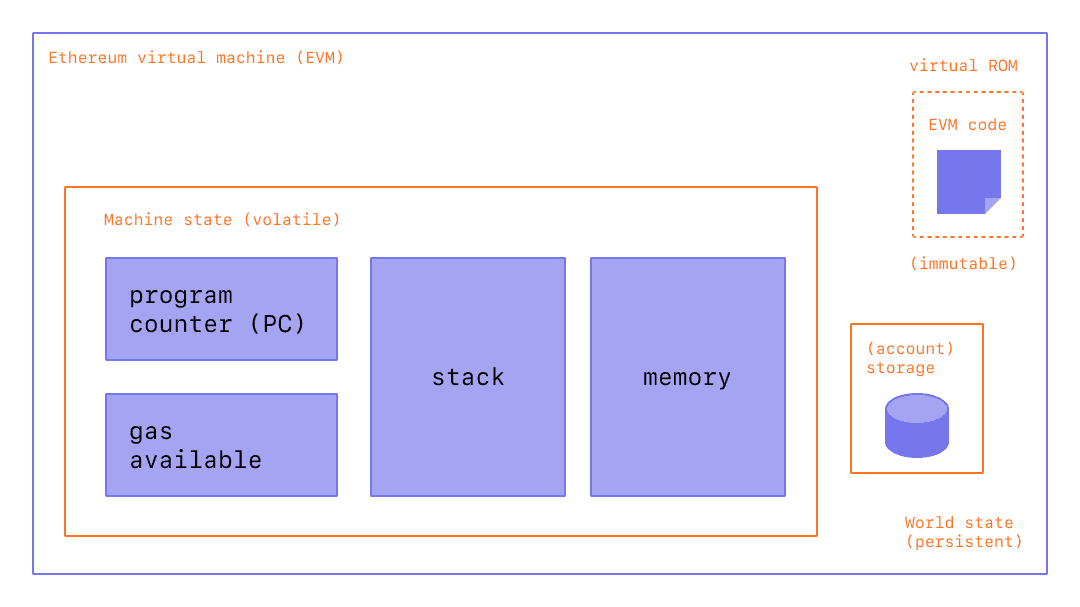
\includegraphics[scale = 0.4]{Figure/evm.png}
    \caption{Sơ đồ kiến trúc EVM (theo \cite{ethereumWhitePaper})}
    \label{fig:evm}
\end{figure}

Ta thấy trên hình \ref{fig:evm} máy ảo có bộ nhớ memory, stack, PC, ROM, storage giống như một máy tính thông thường. Mỗi hợp đồng thông minh trước khi được triển khai lên mạng sẽ được biên dịch dưới dạng bytes code. Phần logic code tức là các hàm (function) sẽ được lưu trữ tại EVM code, đây sẽ là phần không được thay đổi một khi đã được khởi tạo. Các trạng thái của hợp đồng thông minh sẽ được lưu trữ tại storage. Chi tiết về hợp đồng thông minh em sẽ trình bày ở phần sau của phụ lục này.

Trạng thái của máy ảo Ethereum (Ethereum world state) là tập các ánh xạ từ một địa chỉ tới một tài khoản. Trong cài đặt của Ethereum, địa chỉ được tính từ khóa công khai của người dùng đối với tài khoản người dùng. Đối với địa chỉ của hợp đồng được tính từ địa chỉ người triển khai hợp đồng và số nonce của tài khoản triển khai.

\begin{figure}[h!]
    \centering
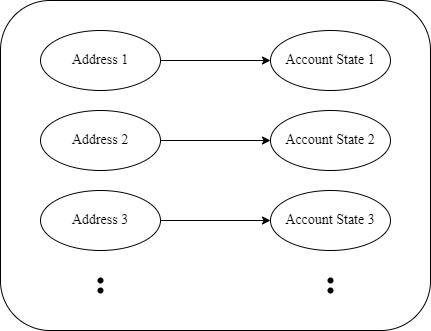
\includegraphics[scale = 0.7]{Figure/worldState.png}
    \caption{Trạng thái của máy ảo Ethereum}
    \label{fig:worldState}
\end{figure}


\section{Các tài khoản}

Trong thế giới Ethereum có hai loại tài khoản (Account). Đó là tài khoản thuộc quyền sở hữu của người dùng (External Owner Account) và hợp đồng thông minh (Smart contract). 

Về điểm chung cả hai loại tài khoản đều có chức năng như:
\begin{enumerate}
    \item Nhận và gửi ETH, các đồng token.
    \item Tương tác với các contract đã được triển khai lên mạng.
\end{enumerate}

Mỗi tài khoản trên mạng Ethereum đều có bốn trường thông tin:
\begin{enumerate}
    \item nonce: Đếm số transaction được gửi từ account, đối với contract account thì đếm số contract được tạo mới bởi nó.
    \item balance: Số wei (đơn vị của ether) được giữ bởi account.
    \item storage root: Giá trị băm của root node Merkle Patricia trie - cấu trúc dữ liệu để lưu trữ trên Ethereum. 
    \item code hash:Giá trị hàm băm của contract code.
\end{enumerate}
Chú ý rằng đối với tài khoản người dùng thì hai trường thông tin storage root và code hash là mặc định.
\begin{table}[h!]
    \centering
    
    \begin{tabular}{||c c||}
    \hline
    Tài khoản người dùng        & Hợp đồng thông minh   \\
    \hline \hline
    Tạo tài khoản miễn phí      & Mất phí triển khai hợp đồng   \\
    Bắt đầu một transaction     & Không thể bắt đầu một transaction \\
    \begin{tabular}{c}
        Transactioin giữa hai người \\
        chỉ có thể là ETH/token
    \end{tabular}  & \begin{tabular}{c}
        Transaction giữa người dùng\\
        và hợp đồng thông mình có thể là \\
        kích hoạt code, tạo hợp đồng mới...
    \end{tabular}\\
    \hline
    \end{tabular}
    \caption{Bảng so sánh tài khoản người dùng và tài khoản hợp đồng}
    \label{table:compareEOAvsCA}
\end{table}


Việc hiểu rõ cấu trúc của các loại tài khoản là cần thiết đối với xây dựng mô hình oracle trả về số ngẫu nhiên trong đồ án này.

\section{Transaction}
Transaction là thông điệp (message) đã ký được gửi từ External owner account (EOA). Transaction sẽ được gửi đến ethereum network xác thực và gộp vào thành một block. Transaction có thể gọi là một hàm chuyển trạng thái trong trạng thái máy ảo (state machine). Và chỉ có transaction mới làm thay đổi trạng thái máy ảo (\ref{fig:transaction}).
\begin{figure}[h!]
    \centering
    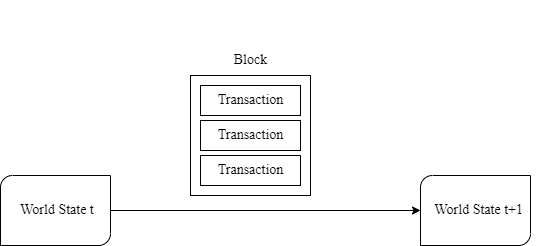
\includegraphics[scale = 0.7]{Figure/transaction.png}
    \caption{Transaction}
    \label{fig:transaction}
\end{figure}
Có hai loại transaction đó là:
\begin{enumerate}
    \item Triển khai, tạo hợp đồng thông minh mới tới tài khoản hợp đồng (Contract creation).
    \item Gọi thông điệp tới các tài khoản, cả tài khoản người dùng và tài khoản hợp đồng (Message call).
\end{enumerate}

Đối với transaction tạo hợp đồng mới, phần code khởi tạo sẽ tạo ra hợp đồng thông minh mới được lưu trên trạng thái máy ảo với logic hợp đồng được lưu tại EVM code, các trường thuộc tính được lưu tại bộ nhớ lâu dài (storage).

Đối với transaction tương tác với hợp đồng đã được triển khai, dữ liệu đầu vào sẽ tương tác với logic code được lưu ở trên EVM code, thực thi và lưu giá trị (nếu có) vào bộ nhớ lâu dài (storage).

Bảng \ref{fig:transaction} cho thấy các thành phần cấu tạo nên một transaction.
\begin{table}[h!]
    \centering
    \begin{tabular}{||l l||}
    \hline
    \multicolumn{2}{c}{Transaction}  \\
    \hline \hline
    nonce       & Số dùng một lần\\
    gasPrice    & Giá của một đơn vị gas (wei)\\
    gasLimit    & Số lượng gas tối đa cho transaction\\
    to          & Địa chỉ nhận transaction (0 nếu khởi tạo hợp đồng)\\
    value       & Số lượng ether gửi cho người nhận\\
    v,r,s       & Chữ ký transaction\\
    init or data& Dữ liệu gửi kèm transaction\\
    \hline
    \end{tabular}
    \caption{Các thành phần của một transaction}
    \label{table:transaction}
\end{table}
\section{Oracle}
Oracles là những hệ thống có thể cung cấp nguồn dữ liệu bên ngoài cho các hợp đồng thông minh Ethereum. Thuật ngữ 'Oracle' xuất phát từ thần thoại Hy Lạp, nơi nó dùng để chỉ một người giao tiếp với các vị thần, người có thể nhìn thấy tầm nhìn về tương lai. Trong bối cảnh của blockchain, oracle là một hệ thống có thể trả lời các thông tin bên ngoài Ethereum. Các oracles là các hệ thống không đáng tin cậy vì chúng hoạt động trên các nguyên tắc tập trung.

Tuy nhiên ý tưởng về mạng các oracle đã được đề xuất từ trước để khắc phục yếu điểm tập trung của hệ thống, phù hợp với nguyên tắc phi tập trung của mạng chuỗi khối.
\section{DAO}
DAO (Decentralized autonomous organizations) là một cách an toàn để làm việc với một nhóm người có cùng mục tiêu. Không một cá nhân nào có quyền ra quyết định mà không được sự chấp thuận của nhóm. Mỗi hành động phải được đề xuất và bình chọn, điều này đảm bảo rằng bất cứ ai trong nhóm đều có thể tham gia vào quyền điều hành.


\end{document}


